% chap4.tex (Customer Description)

\chapter{Customer Description} 

In this chapter, I describe in more detail the customer models implemented in the Power TAC simulation system, and present some descriptive statistics about their behaviors as an initial analysis to indicate important features for learning.

\section{Customer Categories}


In the Power TAC simulation, a customer can be electricity consumer or producer based on its power type. A customer evaluates the tariff plans targeted for its power type and can look for the tariff that minimizes its cost. There are several types of customers in the Power TAC simulation such as consumption, interruptible consumption, thermal storage, solar production, wind production and electric vehicle. Each power type has its own characterstics. For example, interruptible consumption customers can shift their electricity demand to some off peak hour, the solar production customers can produce energy based on the weather condition. As opposed to previous methods of demand forecasting, I argue that each category of customers should have different load forecasting mechanism based on their power types. One load forecasting method can be suitable for a category of customers while it may be unsuitable for other categories because each category behaves differently. I describe the characterstics of the customers below.

\begin{itemize}
\item \textbf{Consumption: } Customers with power type consumption are the most common customers. They use energy when they need it. They cannot shift their demand to a future timeslot. Usually, they have a regular electricity usage pattern. Often, they show a similar pattern for weekdays, and they have similar kind of usage pattern for the weekends. 


\item \textbf{Interruptible Consumption: }
Interruptible consumption customers are smart enough to shift their energy demand in a timeslot where they can buy electricity at a reduced price. Because of this shifting capability, they don't show as regular a usage pattern as the consumption customers do. 

\item \textbf{Thermal Storage: }
Thermal storage customers can store electricity and can supply the stored electricity to the grid depending on its charge level. During a day, their electricity usage in a day depends  much on the energy they used in the last timeslot. 


\item \textbf{Solar Production}
The solar energy production customer's energy production depends on the cloud cover. They are highly likely to produce energy during the day time.

\item\textbf{Wind Production} Wind production customers generate energy from the wind. Their production varies with wind speed.
\item \textbf{Electric Vehicle} An electric vehicle customer represents one electric vehicle. Their usage of energy is quite irregular and hard to predict. \\
\end{itemize}

Before diving into the problem of identifying good forecasting methods, I found it useful to take a look at how the customers of different power types behave. I wrote a log extractor program that extracts all the electricity consumption and production data by all the customer for all of the timeslots. At the end of the game, it makes a report on normalized usage of all the customers. Normalized values are useful because even if the amount of energy usage among the customers varies, the pattern of usage can be captured through it and normalized usages of different customers can be plotted on the same graph. Figures \ref{fig:daily1} to \ref{fig:daily3} show normalized electricity demand or supply for Mondays. 0 in the x axis means hour 12:00 am. From Figures \ref{fig:daily1} to \ref{fig:daily3}, it is clear that some customer's electricity usage is higly correlated with the hour of the day. The customers of type consumption and solar energy are example of these types. The other customer type demands did not have strong correlation with the hour of a day. In both consumption and solar energy customers the consumption or production curve grows fairly smoothly until it reaches a peak point. After the reaching the peak, the production or consumption drops smoothly. The customers with types interruptible consumption, wind production, thermal storage and electric vehicle had irregular demand/supply pattern. 

In figure \ref{fig:weekly1} to \ref{fig:weekly3}, normalized electricity usages during the week are shown. Hour 0 to 23 represents all the hours of Monday from 12:00 am to 11:00 pm. It appears that the electricity demand for consumption customer, interruptible consumption, thermal storage had repetative demand patterns every day. The  solar energy production customer showed repetative production pattern. Moreover some customers such as the consumption type and the thermal storage type showed different pattern during the weekend. During the weekend they usually had lower energy demand than the weekdays. In the case of electric vehicle and wind energy production customers the demand/supply patterns were not regular. From these observations, I assume that the consumption customer and the solar energy type customers can be forecasted with the most accuracy. Due to the irregular patterns of other customers, it will be harder to make accurate demand forecasts about them.
 
% figure start
\begin{figure}
\centering
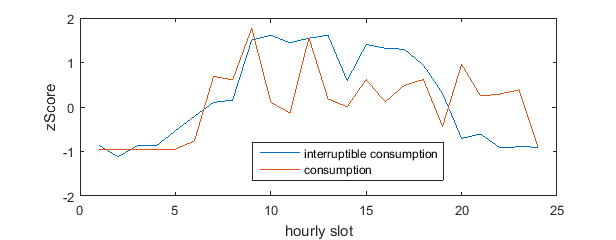
\includegraphics[scale=0.9]{daily1.png}
\caption{energy usage z Score over Monday}
\label{fig:daily1}
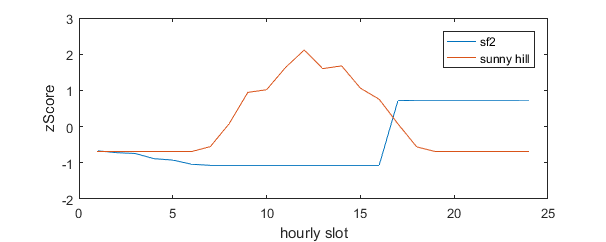
\includegraphics[scale=0.9]{daily2.png}
\caption{electricity usage z Score over Monday}
\label{fig:daily2}
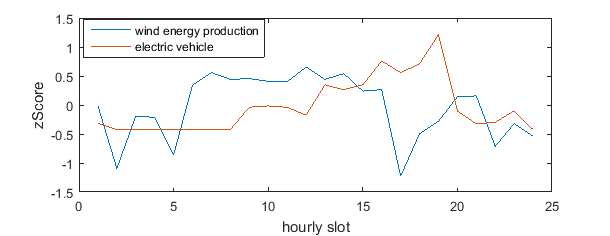
\includegraphics[scale=0.9]{daily3.png}
\caption{electricity usage z Score over Monday}
\label{fig:daily3}
\end{figure}

\begin{figure}
\centering
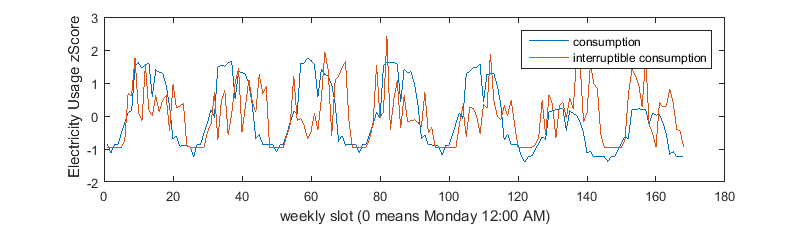
\includegraphics[scale=0.85]{weekly1.png}
\caption{electricity usage z Score over week}
\label{fig:weekly1}
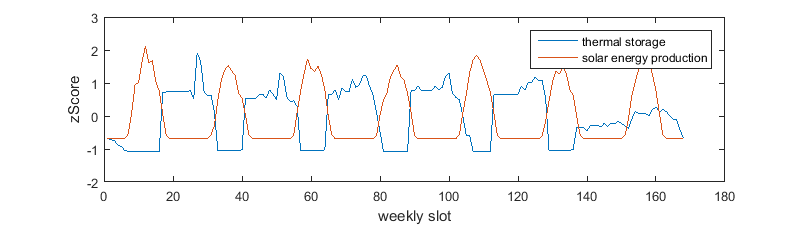
\includegraphics[scale=0.85]{weekly2.png}
\caption{electricity usage z Score over week}
\label{fig:weekly2}
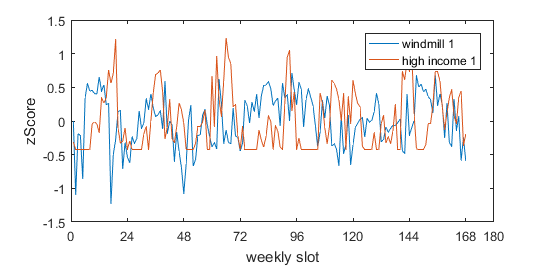
\includegraphics[scale=0.85]{weekly3.png}
\caption{electricity usage z Score over week}
\label{fig:weekly3}
\end{figure}

%figure end

\section{Statistics}
In this section, I present some descriptive analysis of the customers available in the system to get an initial understanding of the typical behavior of the models. 

\begin{itemize}
\item \textbf{Customer Vs PowerType}

The figure \ref{fig:cust-pt} shows number of customers of each power type for a typical Power TAC simulation game. The electric vehicle power type has the largest number of customers. This is because each electric vehicle represents a population of size 1. Consumption and interruptible consumption power type customers follow the electric vehicle power type customers in terms of number of customers. 

\item \textbf{Population Vs PowerType}
From figure \ref{fig:pop-pt} the power type of consumption has by far the largest number of population. Some customers can represent thousands of individuals. For this reason, even though there are only a few numbers of consumption and solar energy customers, they can represent a population of several thousand individual customer households. 

\item \textbf{Total Energy Consumed Vs PowerType}
The Figures \ref{fig:energy-pt} and \ref{fig:energy-shares} show the contribution to energy transactions by different power type customers in a typical Power TAC simulation. From the figure, we can see that the consumption type customers are responsible for the largest amount of energy transaction of total quantity (more than 60\%). After the consumption type customers, the interruptible consumption type customers trade 18\% of total traded energy. The solar production customers had 11\% of the total energy transactions. A successful broker needs to forecast the consumption type customer with prime importance because of the bulk of energy they transact. Due to this fact, I concentrated mostly on forecasting about consumption type customer demand.


\begin{figure}
\centering
\begin{minipage}{.5\textwidth}
  \centering
  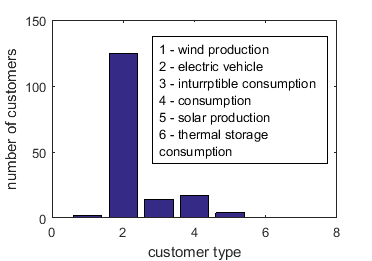
\includegraphics[width=\linewidth]{4-customer-vs-powertype.png}
  \caption{Number of customers vs Powertype.}
  \label{fig:cust-pt}
\end{minipage}%
\begin{minipage}{.5\textwidth}
  \centering
  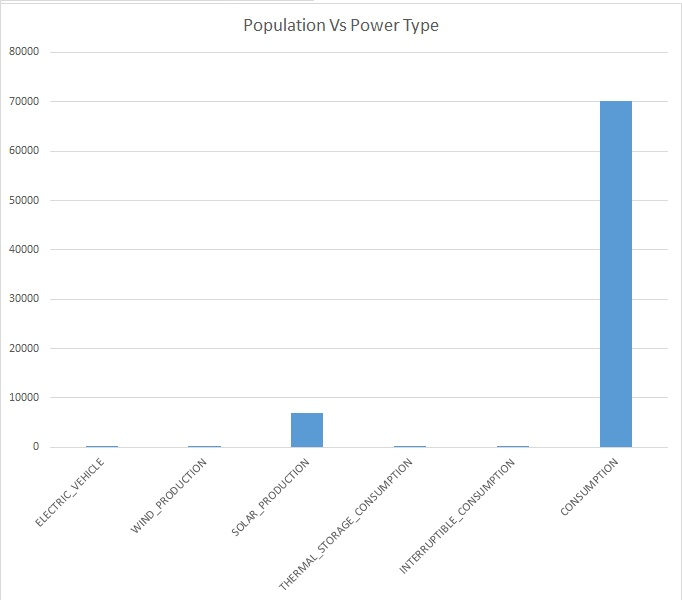
\includegraphics[width=\linewidth]{2-population-vs-powertype.jpg}
  \caption{Population vs Powertype}
  \label{fig:pop-pt}
\end{minipage}

\centering
\begin{minipage}{.5\textwidth}
  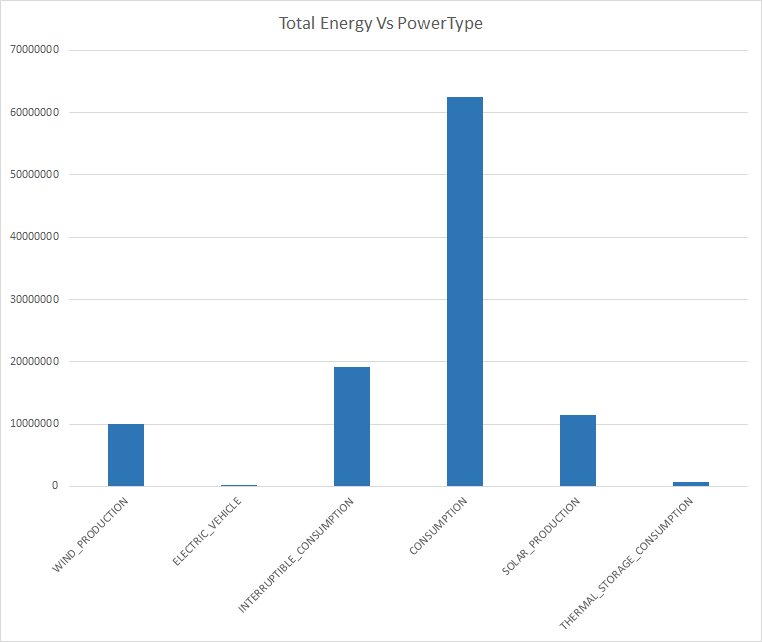
\includegraphics[width=\linewidth]{3-energy-vs-powertype.png}
  \caption{Energy vs PowerType.}
  \label{fig:energy-pt}
\end{minipage}%
\begin{minipage}{.5\textwidth}
  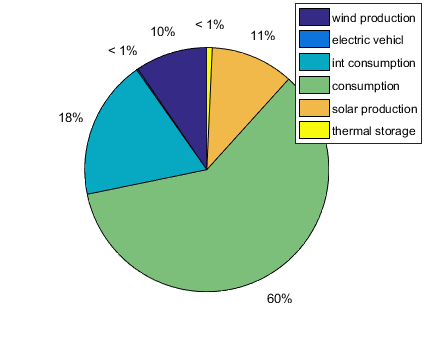
\includegraphics[width=\linewidth]{pie-energy-share.png}
  \caption{Energy share for each power type.}
  \label{fig:energy-shares}
\end{minipage}

\end{figure}

\end{itemize}
